\documentclass[10pt,a4paper]{article}

\usepackage{geometry}
\geometry{left=1cm, right=1cm, top=0.6cm, bottom=0.6cm}

\usepackage{fontspec}
\usepackage{xcolor}
\usepackage{enumitem}
\usepackage{fontawesome5}
\usepackage{graphicx}
\usepackage{fancyhdr}

\setmainfont{Arial}

% Adjust line spacing and paragraph spacing
\linespread{1.18} % Slightly reduced from 1.2 to fit English text
\setlength{\parskip}{0.15ex}

% Color definitions
\definecolor{myblue}{RGB}{74,118,206}
\definecolor{tagblue}{RGB}{120,150,220}
\definecolor{tagbg}{RGB}{240,245,255}

\pagestyle{empty}

\newcommand{\cvsection}[2]{
  \vspace{0.5ex}
  \noindent{\color{myblue}\Large\bfseries\faIcon{#1}\hspace{0.5em}#2} \textcolor{myblue!50}{\hrulefill}\par
  \vspace{0.2ex}
}

\newcommand{\cvtag}[1]{%
  \raisebox{0.1ex}{%
    \setlength{\fboxsep}{1.5pt}%
    \colorbox{tagbg}{\textcolor{tagblue}{\fontsize{11pt}{13.2pt}\selectfont #1}}%
  }%
  \hspace{0.2em}%
}

% Custom list indentation and spacing
\setlist[itemize,1]{leftmargin=0pt, label=, itemsep=0.4ex, topsep=0.4ex, parsep=0pt}
\setlist[itemize,2]{leftmargin=0.7em, label=$\circ$, itemsep=0.2ex, topsep=0.2ex, parsep=0pt}

\begin{document}

\vspace*{-0.6cm}
\begin{center}
  \textbf{\LARGE MA CHIYUAN}\\[0.5ex]
  13191869708 ~|~ machiyuan6@163.com ~|~ 2002-12 ~|~ Male
\end{center}

\begin{picture}(0,0)
  \put(440, 7){
    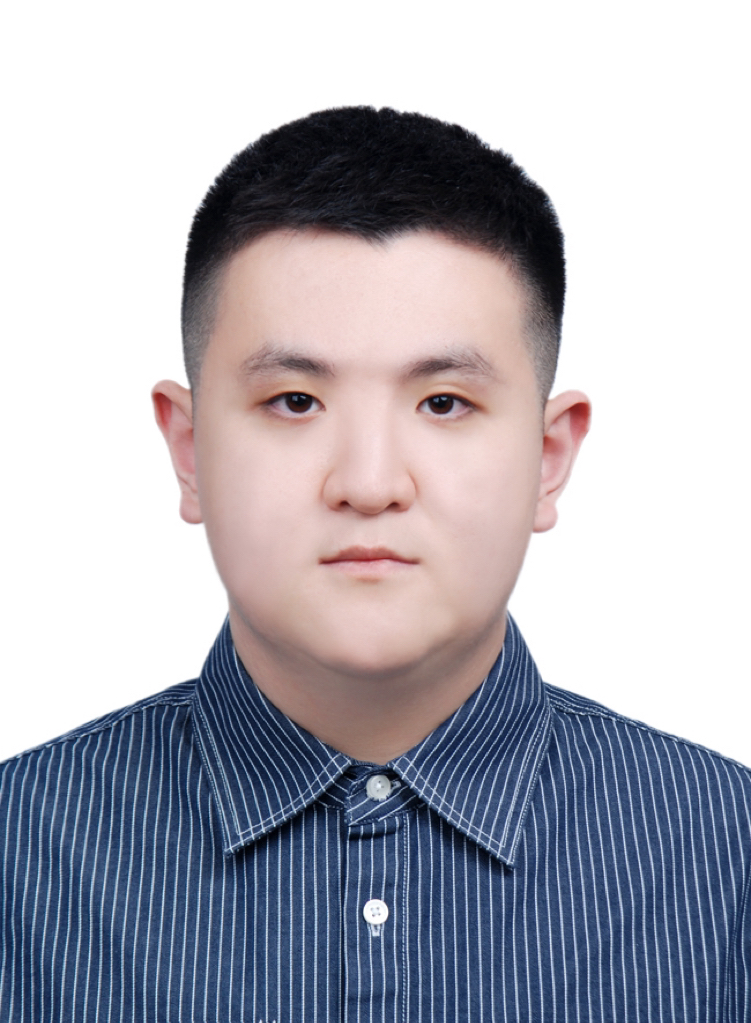
\includegraphics[height=2.4cm, keepaspectratio]{本科毕业证件照.jpg}
  }
\end{picture}

\vspace*{-1.2cm}

% Education
\cvsection{graduation-cap}{Education}

{\fontsize{12pt}{14.4pt}\selectfont\noindent\textbf{Northeastern Univ. (NEU)} - B.S. App. Statistics \hspace{0.5em} \cvtag{985} \cvtag{211} \cvtag{D-First-Class} \hfill 2021.09 - 2025.07\par}
\begin{itemize}[leftmargin=1em, label=, itemsep=0.35ex, topsep=0.05ex]
\item \textbf{[GPA \& Courses]} \textbf{GPA: 3.7/4.0}; Courses: Python, Math, Probability, Deep Learning, Simulation, etc.
\item \textbf{[Information Security Lab]} Advisor: \textbf{Prof. Shi Wenbo}; Assisted in building blockchain contract simulation systems; Studied distributed architecture and Lake-Warehouse unified systems.
\end{itemize}
\vspace{0.2ex}

{\fontsize{12pt}{14.4pt}\selectfont\noindent\textbf{Nanyang Tech. Univ. (NTU)} - M.S. Signal Proc. \& ML \hspace{0.5em} \cvtag{QS\#12} \cvtag{US\#28} \hfill 2025.08 - 2026.08\par}
\begin{itemize}[leftmargin=1em, label=, itemsep=0.35ex, topsep=0.05ex]
\item \textbf{[Courses \& Research]} \textbf{GPA: 3.9/5.0}; CV, ML, Video Signal Proc.; \textbf{Adv.: Assoc. Prof. Z. Lin}.
\end{itemize}

% Experience
\cvsection{briefcase}{Experience}

{\fontsize{12pt}{14.4pt}\selectfont\noindent\textbf{A*STAR} - I2R - Research Assistant \hfill 2025.09 - 2026.07\par}
\begin{itemize}[leftmargin=1em, label=, itemsep=0.35ex, topsep=0.05ex]
\item \textbf{[Project Lead]} Led development of \textbf{MHR-based Precise AI Guidance System} for sports training/therapy; 
\item \textbf{[Architecture]} Designed workflows; Proposed \textbf{Dual-Track Spatial Decoupling Architecture \& Cross-Attention} fusing 2D pose/3D camera data, cutting drift by \textbf{38\%}.
\item \textbf{[Kinematic Super-Resolution]} Developed generative MLP model on \textbf{68D One-hot} encoding to upsample 17 sparse markers to full 6DOF skeletal rotation; Reduced keypoint error by \textbf{50\% (to 0.6 mm)} with \textbf{CPU inference >200 Hz}.
\item \textbf{[Optimization]} Decoupled body shape/pose via multi-stage models; Integrated \textbf{Adaptive Scale}, \textbf{Confidence-Weight PnP}, and \textbf{Kalman Filter}; Achieved \textbf{4.2 mm} error and \textbf{<5 ms} latency on 2.7k+ frames, supporting \textbf{>30 fps}.
\end{itemize}
\vspace{0.2ex}

{\fontsize{12pt}{14.4pt}\selectfont\noindent\textbf{JD.com} - B2B Sourcing Ops - Govt \& Enterprise Innovation \hfill 2024.08 - 2025.04\par}
\begin{itemize}[leftmargin=1em, label=, itemsep=0.35ex, topsep=0.05ex]
\item {\fontsize{10.5pt}{12pt}\selectfont\textbf{[Model Operations]}} \textbf{Optimized scoring models, shifting workflows from manual to objective quantification.}
  \begin{itemize}
    \item Discovered issues in B2B onboarding mismatching retail standards and lack of supplier quantitative monitoring.
    \item Reshaped workflows with PMs and created guides, increasing \textbf{OKR by 17\% YoY} and cutting lead time from \textbf{38h to 27h}.
    \item Built a \textbf{Python} multi-factor model to identify/eliminate 38 inactive suppliers, boosting revenue by \textbf{13\%}.
  \end{itemize}
\item {\fontsize{10.5pt}{12pt}\selectfont\textbf{[Efficiency Tools 0-1]}} \textbf{Identified pain points and developed internal tools end-to-end.}
  \begin{itemize}
    \item Developed "Sourcing Assistant" (WeChat plugin) using \textbf{Python}; Integrated Yanxi LLM; Designed multi-layer security \& prompt isolation; Achieved low-latency streaming and high reliability (100k+ cumulative replies).
    \item Developed an automated invoice recognition system (OCR, masking, archiving); Handled \textbf{15k+ invoices}, saving \textbf{400 man-days} during sales peaks with \textbf{300\% efficiency gain}; Packaged as EXE for departmental use.
    \item Built crawlers for client order extraction, fetching 3000+ records (~300k CNY) complying with robot protocols.
  \end{itemize}
\end{itemize}
\vspace{0.2ex}

{\fontsize{12pt}{14.4pt}\selectfont\noindent\textbf{HBIS Group SCM} - Data Analyst - Platform Ops \hfill 2024.05 - 2024.08\par}
\begin{itemize}[leftmargin=1em, label=, itemsep=0.35ex, topsep=0.05ex]
\item \textbf{[Evaluation Modeling]} Set risk metrics and IAHP models for steel plants, supporting 3 platforms with 0 operational errors.
\item \textbf{[Data Management]} Used \textbf{SQL} for deep cleaning and outlier analysis of logistics freight data, capturing 18 abnormal fluctuations; Executed 77 complex data extractions, ranking \textbf{1st in team} for efficiency, precision, and data quality.
\item \textbf{[Operations]} Maintained \textbf{Efree} platform, resolving 300+ compliance cases; Supported data certification and financing.
\end{itemize}

% Projects
\cvsection{star}{Projects \& Competitions}

{\fontsize{12pt}{14.4pt}\selectfont\noindent\textbf{Privacy Compliance for Lake-Warehouse Data Analysis} \hfill 2022.03 - 2023.12\par}
\begin{itemize}[leftmargin=1em, label=, itemsep=0.35ex, topsep=0.05ex]
\item \textbf{[Framework]} Designed comprehensive lake-warehouse based privacy framework involving verification, TEE, and cross-chain blockchain layers; Introduced reputation-based penalties, reducing unauthorized analysis by \textbf{36\%} across systems.
\item \textbf{[Data Analysis]} Collected 300+ runtime data points to identify 36 bottlenecks; Assisted student validation with 3G+ data.
\item \textbf{[Outputs]} Ma, C., \& Hu, X. (2023). Privacy Compliance for Lake-Warehouse Analysis. \textit{ACM ADMIT 2023}.
\item \textbf{[Innovation]} Granted a \textbf{Chinese Invention Patent}, validating its practical and innovative value.
\end{itemize}
\vspace{0.2ex}

{\fontsize{12pt}{14.4pt}\selectfont\noindent\textbf{Public Willingness for Hospice Care in Qinhuangdao} \hfill 2022.12 - 2023.08\par}
\begin{itemize}[leftmargin=1em, label=, itemsep=0.35ex, topsep=0.05ex]
\item \textbf{[Data Collection]} Investigated acceptance; Collected 632 questionnaires via \textbf{web crawling} and \textbf{sampling}.
\item \textbf{[Modeling]} Built multi-weight evaluation model using \textbf{Logist RG, PCA, Random Forest, K-means}, \textbf{78\% accuracy}.
\item \textbf{[Awards]} \textbf{National 3rd Prize} in the 13th CICAS; \textbf{Provincial 2nd Prize} in the 9th National Statistics Modeling Contest.
\end{itemize}

% Personal
\cvsection{user}{Personal Details}

\begin{itemize}[leftmargin=0pt, label=, itemsep=0.3ex, topsep=0.3ex]
\item \textbf{[Honors]} 5x School Scholarships (3rd); 2x Innovation \& Entr. (23\&24); Outstanding Leader; Outstanding Student.
\item \textbf{[Skills]} \textbf{Python(Pandas/NumPy) > SQL > SPSS}; Proficient in \textbf{AI-Coding} (Antigravity), Prompt Engineering, and RAG architectures; Completed Tencent PM Camp with focus on user-centric product thinking and growth strategies.
\item \textbf{[Self-Evaluation]} Outgoing; Capable of working under pressure; Strong coordination and communication skills; Fast learner.
\end{itemize}

\end{document}
